\documentclass[11pt,oneside,final,showtrims]{memoir}

\makeatletter
\usepackage{soul}
\usepackage[cmyk]{xcolor}

\usepackage[pdftex]{graphicx}
\graphicspath{{../../assets/Images/}}

\usepackage{calc}
\usepackage{xcoffins}

\newif\ifvarnishmask
\varnishmaskfalse

\newlength\BOOK@tmp@width
\newlength\BOOK@tmp@height

% #1 -- the commands to hold the place for
\newcommand\placeholder[1]{%
\ifvarnishmask%
\settowidth{\BOOK@tmp@width}{#1}%
\settototalheight{\BOOK@tmp@height}{#1}%
{\color{black}\rule{\BOOK@tmp@width}{\BOOK@tmp@height}}%
\else%
#1%
\fi%
}

% === setup page layout ===

\newlength\BOOK@paperHeight
\newlength\BOOK@paperWidth
\setlength{\BOOK@paperHeight}{120mm}
\setlength{\BOOK@paperWidth}{135mm}

\ifshowtrims
  \setstocksize{\BOOK@paperHeight+30mm}{\BOOK@paperWidth+30mm}
  \setlength{\paperheight}{\BOOK@paperHeight}
  \setlength{\paperwidth}{\BOOK@paperWidth}
  \trimXmarks
  \trimLmarks
  \quarkmarks
  \settrims{0.5\stockheight - 0.5\paperheight}{0.5\stockwidth - 0.5\paperwidth}
  \settrimmedsize{\BOOK@paperHeight}{\BOOK@paperWidth}{*}
\else\relax
  \setstocksize{\BOOK@paperHeight}{\BOOK@paperWidth}
  \settrimmedsize{\stockheight}{\stockwidth}{*}
  \settrims{0pt}{0pt}
\fi

\setlrmarginsandblock{0pt}{0pt}{*}
\setulmarginsandblock{0pt}{0pt}{*}
\setheaderspaces{*}{0pt}{*}
\setheadfoot{0pt}{-10pt}

\checkandfixthelayout% This will typeout values in pt.
\settypeoutlayoutunit{mm}% It is useful to see layout values in mm too.
\typeoutlayout

\usepackage{fontspec}
\setmainfont[Ligatures = TeX]{Shaker 2 Light}

\newfontfamily\titleFont[Ligatures = TeX]{Shaker 2 Light}
\newfontfamily\authorFont[Ligatures = TeX]{Shaker 2 Light}
\newfontfamily\volumeFont[Ligatures = TeX]{Shaker 2 Regular}

\sodef\soTitle{}{.1em}{.5em plus.1em}{.1em plus.1em minus.1em}
\sodef\soAuthor{}{.1em}{.5em plus.1em}{.1em plus.1em minus.1em}
\sodef\soVolume{}{.4em}{1.2em plus.1em}{.1em plus.1em minus.1em}

\newcommand\titleSize{\@setfontsize\titleSize{18}{19}}
\newcommand\volumeSize{\@setfontsize\volumeSize{10.5}{11}}

\usepackage[final]{microtype}

\newlength\bleed
\setlength{\bleed}{1mm}

\NewCoffin\CoverWrap
\NewCoffin\Photo
\NewCoffin\Title
\NewCoffin\Author

\newlength\photoWidth
\newlength\authorWidth

\setlength{\photoWidth}{95mm}
\setlength{\authorWidth}{38mm}

\pagestyle{empty}

\setlength{\parindent}{0pt}
\makeatother

\begin{document}

\centering

\makeatletter
\SetHorizontalCoffin\Photo{%
\placeholder{%
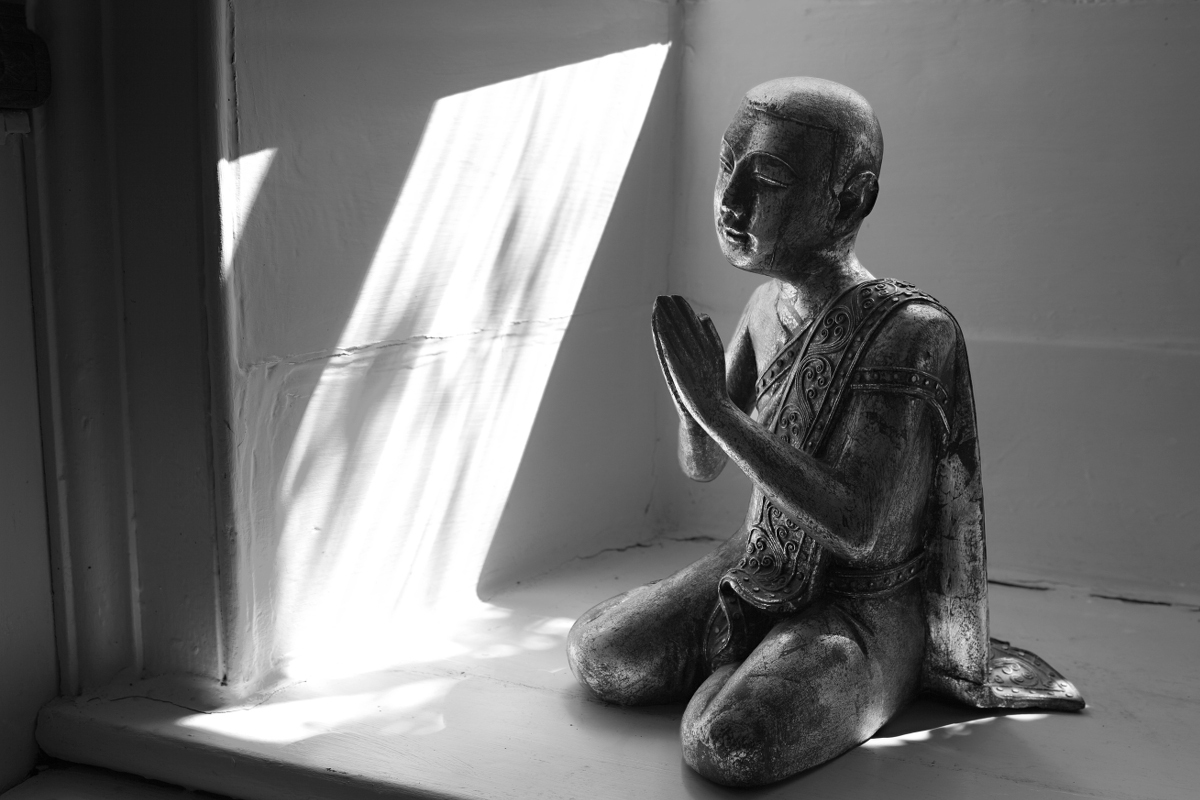
\includegraphics[width=\photoWidth,keepaspectratio]{cover_photo.jpg}%
}%
}%

\SetHorizontalCoffin\Title{%
  \resizebox{\photoWidth}{!}{\titleFont\titleSize\color[gray]{0.35}\soTitle{Dhammapada Reflections}}%
}%

\SetHorizontalCoffin\Author{%
\begin{minipage}{\linewidth}%
  \centering
  \resizebox{\authorWidth}{!}{\authorFont\color[gray]{0.35}\soAuthor{Ajahn Munindo}}\\
  {\color[gray]{0.3}\rule[6pt]{\authorWidth}{0.25pt}}\\
  \vspace*{-7pt}%
  {\volumeFont\volumeSize\color[gray]{0.75}\soVolume{Volume Three}}
\end{minipage}%
}%

\JoinCoffins*\CoverWrap[hc,t]\Photo[hc,b](0pt,-57.5mm)%
\ifvarnishmask\relax
\else
\JoinCoffins*\CoverWrap[hc,t]\Title[hc,t](0pt,-60mm)%
\JoinCoffins*\CoverWrap[hc,t]\Author[hc,t](0pt,-98mm)%
\fi
\makeatother

\TypesetCoffin\CoverWrap%

\end{document}
